\documentclass[a4paper]{article}

%% Language and font encodings
\usepackage[english]{babel}
\usepackage[utf8x]{inputenc}
\usepackage{colortbl}
\usepackage[T1]{fontenc}

%% Sets page size and margins
\usepackage[a4paper,top=3cm,bottom=2cm,left=3cm,right=3cm,marginparwidth=1.75cm]{geometry}

%% Useful packages
\usepackage{amsmath}
\usepackage{graphicx}
\usepackage[colorinlistoftodos]{todonotes}
\usepackage[colorlinks=true, allcolors=blue]{hyperref}

\title{Initial Report}
\author{Written by : GoChat Team}

\begin{document}
\maketitle

%\begin{abstract}
%Your abstract.
%\end{abstract}

\section{Introduction}

Nowadays, with rapid development of the digital technologies, distributed chat systems play an increasingly indispensable role in people’s daily life. They provide a way for people with geographical barriers to communicate, to study, to work together. 
Our project, go-chat, is an example of distributed chat systems, which allows users on two clients to enjoy basic features (add their friends, send messages, make group chats and etc.) and additional features (make notes, send emotion, download history and etc.) without compromising their privacy. It consists of two clients, windows desktop application and web page, and one server. C\# and PHP are chosen as the programming languages for the windows desktop application and web page respectively. And WebSocket Protocol is used to ensure the communication between the clients and the server. 



%WebSocket Protocol is used to ensure the communication between clients and server. (The WebSocket is a feature of HTML5 for establishing a socket connections between a web browser and a server, once the connection has been established with the server, all WebSocket data (frames) are sent directly over a socket rather than usual HTTP response and requests, giving us much faster, persistent and full-duplex communication between a web browser and a server.)





%\subsection{Project Scope}



\section{Project Description}

\subsection{Project Structure}

\begin{figure}[h]
\centering
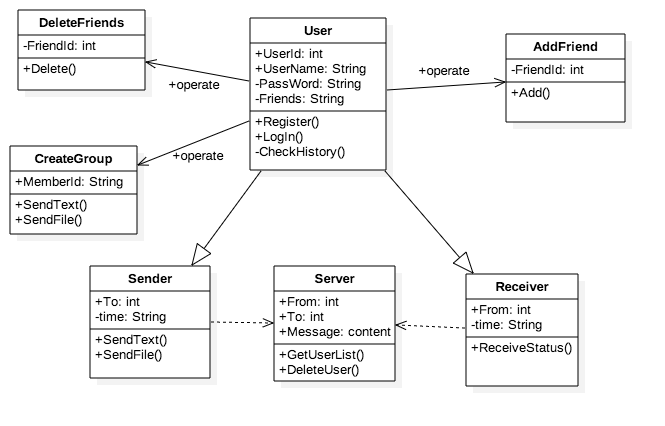
\includegraphics[width = 0.85 \textwidth ]{UML.png}
\caption{\label{fig:UML}UML Class Diagram}
\end{figure}

\subsection{Project's Aims and Strategy to Achieve Our Aims}
Our aim for this project is to build a reliable, secure, and attractive chat system. Reliable in the term that every message sent by client will be received in a relatively real-time. Client would not have to concern about lost message even in a slow network connection or offline case. Meanwhile, secure in this case means that there are no unauthorized principal can read message sent from one client to another client.

In order to achieve those goals, we divided our project into three main level, Basic Chatting Program, Security, and Other Additional Functions. 

\subsubsection{Level 1: Basic Functionalities}

In this level, basic infrastructure will be built for the server and two clients, the web page and the windows desktop application, to achieve basic functionalities for the system. 

\begin{itemize}
%--------------------------------------------------------
%change User




\item Server
\begin{enumerate}
\item Database is used to store users' names, passwords, personal information, friends' information and chatting informations in the server.
\item Apache server is used to make connection between server and clients.
\end{enumerate}


%: Keep chatting record in the database. It store data until the user request to delete history.

%: describe database table(how to store data)

%: it might be depend on option. If someone do not want to store data(like private mode), data will delete when user delete chatting.

% : open web sever by open source program Apache

% : it can be replace by github(github provide storage. it can use as a web server)


\item Client
\begin{enumerate}
\item Clients could set up the connection with server (Figure 2).
\item Client 1 send message to server
\item Client 2 receive message from server which from the client 1.
\item If the the message is not a plane text, client 2 send a request to server to receive data.
\item Client 2 receive data which as picture and document.

\end {enumerate}
\item User

\begin{enumerate}
\item Users on the clients could sign up creating their user names and passwords and also filling in their personal details.
\item Users on the clients could add their friends and send messages (text, files and pictures) to them.
\item Users on the clients could check whether their friends are on line or not.
\item  Users on the clients could create groups with adding their friends to the group and begin group chats.

\end{enumerate}
\end{itemize}
\begin{figure}[h]
\centering
\includegraphics[width = 0.7 \textwidth ]{SC.png}
\caption{\label{fig:UML2}Server/Client Model}
\end{figure}

%\begin{table}[h]
%\caption{Payload}
%\begin{center}
%\begin{tabular}{| c | c | c | c |}
%\hline
%sender & receiver & type & message\\
%\hline
%\end{tabular}
%\end{center}
%\end{table}

% \begin{itemize}
% \item Payload

% - This is a simple version of the payload for communicating between server and client

% - type: provide what type of the message it is. Such as plain text, picture, video, and document.

% - message: If message is a plain text, it contains the text. Another cases (picture, and so on), it contains server storage a URL. Based on the URL, files will be download from the server. 

% \end{itemize}

\subsubsection{Level 2: Security}

Chatting program is private communication. Confidentiality, Privacy, and Integrity are common issues at the chatting program. It contains personal information, photos, business secret, and so on. These kind of information must be encrypted to avoid leakage. For encryption, many solutions are available such as trusted third party protocol or asymmetric keys encryption.

While level 1 provides basic functionalities without considering the security, the aim of the go-chat level 2 is to keep everything secure. In level 1, program store unencrypted history at server. Meanwhile in level 2, it will be encrypted by security protocols, so that only those who participate in the chatting can read their chatting history. In this level, user also should be able to delete their chatting history to prevent data theft. In addition, user can customize message expire time. For example, if user set the expire time to one day, the message will be automatically deleted after 24 hours. The message will be deleted even if the receiver has not seen the message.

In term of security aspect, we will focus on two parts, communication security and security of data storage. For communication security, websocket protocol doesn’t handle the authorization or authentication. However, just like the https which is actually http over TLS, using the WSS (websocket over TLS/SSL) to encrypt our connection can make sure our information transfer security. In this case, we just need to configure TLS encryption for websocket and self-sign the certificate. For database security, we choose to use SALT and hash function to encrypt the username and password to avoid dictionary attacks. Using different encryption algorithm for other data. In this way, we can prevent the SQL injection attack.

\subsubsection{Level 3: Other Additional Functions}

Chatting program have to be attractive. It is not only for sending plane text messages to friend. It has to be possible to explain emotion of the people. That's why people use emojis and photos. In level 3 period, go-chat program contain attractive function such as use emojis, gif, drawing picture, recommend friend, offline message, print history, recall message, and image compose.

\subsection{Time Management}

\definecolor{No}{RGB}{255,255,185}
\definecolor{UML}{RGB}{205,205,180}
\definecolor{Data}{RGB}{205,205,180}
\definecolor{intermediate}{RGB}{205,205,180}
\definecolor{environ}{RGB}{205,205,180}
\definecolor{level1}{RGB}{205,205,180}
\definecolor{level2}{RGB}{205,205,180}
\definecolor{level3}{RGB}{205,205,180}
\definecolor{debug}{RGB}{205,205,180}
\definecolor{documentation}{RGB}{205,205,180}
\definecolor{final}{RGB}{205,205,180}

\begin{table}[h]
\centering
\caption{Task time table}
\label{my-label}
\begin{tabular}{|c|l||c|c|c|c|c|c|c|c|c|c|}
\hline
\rowcolor{No}
No. & Task name & 01 & 02 & 03 & 04 & 05 & 06 & 07 & 08 & 09 & 10 \\ \hline \hline
1 & UML design & \cellcolor{UML} & \cellcolor{UML} &  &  &  &  &  &  &  &  \\ \hline
2 & Database design & \cellcolor{Data} & \cellcolor{Data} &  &  &  &  &  &  &  &  \\ \hline
3 & Intermediate report \& presentation &  & \cellcolor{intermediate} & \cellcolor{intermediate} &  &  &  &  &  &  &  \\ \hline
4 & Developing environment setting &  &  & \cellcolor{environ} & \cellcolor{environ} &  &  &  &  &  &  \\ \hline
5 & Level 1: basic chatting program &  &  & \cellcolor{level1} & \cellcolor{level1} & \cellcolor{level1} &  &  &  &  &  \\ \hline
6 & Level 2: security &  &  &  &  & \cellcolor{level2} & \cellcolor{level2} & \cellcolor{level2} &  &  &  \\ \hline
7 & Level 3: Other additional function &  &  &  &  &  &  & \cellcolor{level3} & \cellcolor{level3} & \cellcolor{level3} &  \\ \hline
8 & Debug &  &  &  &  & \cellcolor{debug} & \cellcolor{debug} & \cellcolor{debug} & \cellcolor{debug} & \cellcolor{debug} & \cellcolor{debug} \\ \hline
9 & Documentation &  &  &  &  & \cellcolor{documentation} &  & \cellcolor{documentation} &  & \cellcolor{documentation} &  \\ \hline
10 & Final report \& presentation &  &  &  &  &  &  &  &  & \cellcolor{final} & \cellcolor{final} \\ \hline
\end{tabular}
\end{table}


\subsection{Initial Progress}
%-----------------------------------------------
% add some description 


We already design the project structure (Figure 1), the database (Figure 3) and make the project plan(timetable). The timetable can be seen in table 1. 

Since storing chat messages and retrieving those messages at a very fast rate is much needed for a chatting software, the MYSQL is used as our database management system and 4 tables will be created to store different sorts of data.


\begin{figure}[h]
\centering
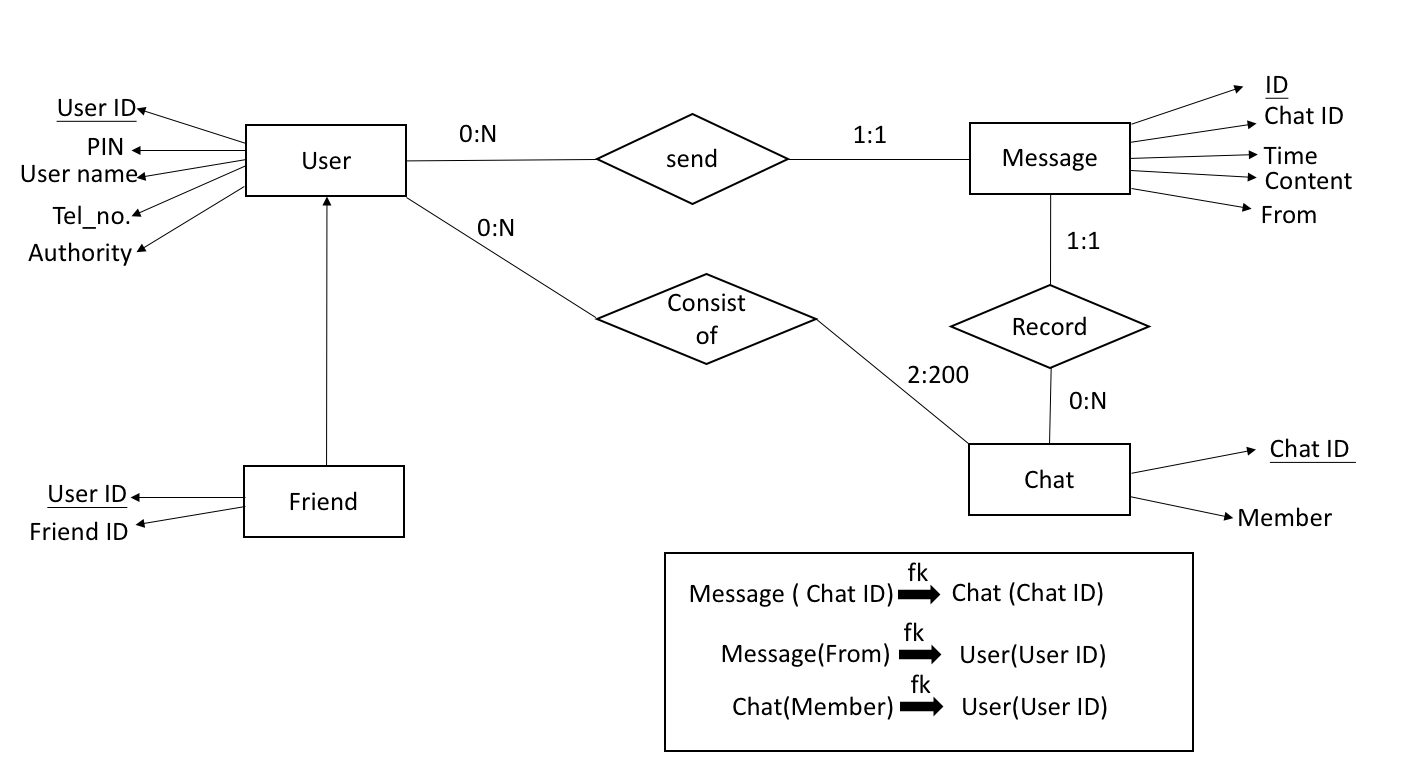
\includegraphics[width = 0.85 \textwidth ]{ERD.png}
\caption{\label{fig:ERD}Entity Relation Diagram}
\end{figure}

\begin{itemize}
\item Table ‘user’ would contain the basic information of all users including userID, password, username etc. 
\item Table ‘friend’ is used to store the userID and the friendID of their friends’.
\item Table ‘message’ will list the detail of every single message including chatID, sending time, content of message, and the sender’s userID.
\item Table ‘chat’ is used to record the member of chatting and their chatID. 
\end{itemize}


\begin{itemize}
\item Key constraint:

Primary key: user(userID), message(ID), friend(userID), chat(chatID).

Foreign key: message(chatID), message(from), chat(member).

\end{itemize}


\section{Project Organization}

\subsection{Roles of Team Members}

We divided our team member into two small teams, web application team and window application team. The first team will build the web client, while the other will build the window client. We also decided to build the server together.

\subsection{How to Collaborate with Each Other (Tools)}

We decided to hold a meeting every Thursday at 19.30 at Guy's Campus Library. In this meeting, we will discuss our progress for the last 7 days and our target for the next week. We will also discuss the problems that might be arisen here. We will use WhatsApp application as our main way of communication. 

\subsection{Peer Assessment}

We believe that we as the member of the group have the same responsibilities for the success of our project. We strongly believe that each of our members will work as hard as they can to ensure this project is a success. That is why we decided to give each of us a 15 mark for our effort. On the other hand, We will divide the rest of 10 marks based on our member's creativity, ability to handle stress and pressure, and the ability to keep our group together.

\subsection{Conflict Handling}

Conflict related to the development of the system will be discuss every week. We will discuss the problem and narrow down the possible solutions. We will also consider the advantages and disadvantages of every option before deciding the best option. 

\end{document}